\documentclass[usenames,dvipsnames]{beamer}
\usepackage[utf8]{inputenc}
\usepackage[T1]{fontenc}
\usepackage[french]{babel}
\usepackage{xcolor}
\usetheme{Singapore} %Boadilla | Bergen | Madrid | Antibes | Hannover | Singapore | Warsaw
%----------------------------------------------------------------------------------------
%   TITLE INFORMATION
%----------------------------------------------------------------------------------------
\title{CourtCircuit}
\subtitle{HLSE602 -- Projet CMI Annuel}
\author{B. Rima \and O. Farajallah \and W. Soussi}
\institute[UM]{L3 CMI Informatique}
\date{\today}

\begin{document}
%----------------------------------------------------------------------------------------
%   TITLE FRAME
%----------------------------------------------------------------------------------------
\begin{frame}
\titlepage
\end{frame}
%----------------------------------------------------------------------------------------
%   OUTLINE
%----------------------------------------------------------------------------------------
\begin{frame}[allowframebreaks]{Sommaire}
    \tableofcontents
\end{frame}
%----------------------------------------------------------------------------------------
%   INTRODUCTION
%----------------------------------------------------------------------------------------
\section{Introduction}
\begin{frame}{Contexte du projet}{Introduction}
  \begin{description}
    \item [Projet CMI :] Module d'un projet annuel pour l'année 2017--2018 dans le cadre du \textbf{CMI Informatique}.
    \item [Responsable CMI Informatique :] Mme Anne-Elisabeth Baert.
    \item [Encadrant du projet :] M. Eric Bourreau.
    \item [Lieux de travail :] La \textbf{FDS} et le \textbf{LIRMM}.
  \end{description}
\end{frame}

%----------------------------------------------------------------------------------------
%   PROBLÉMATIQUE ET MÉTHODOLOGIE DE RÉSOLUTION
%----------------------------------------------------------------------------------------
\section{Problématique et Méthodologie de Résolution}
\subsection{Problématique (Rappels)}
\begin{frame}{Problématique}{Problématique et Méthodologie de Résolution}
\begin{columns}[onlytextwidth, T]
  \column{55mm}
    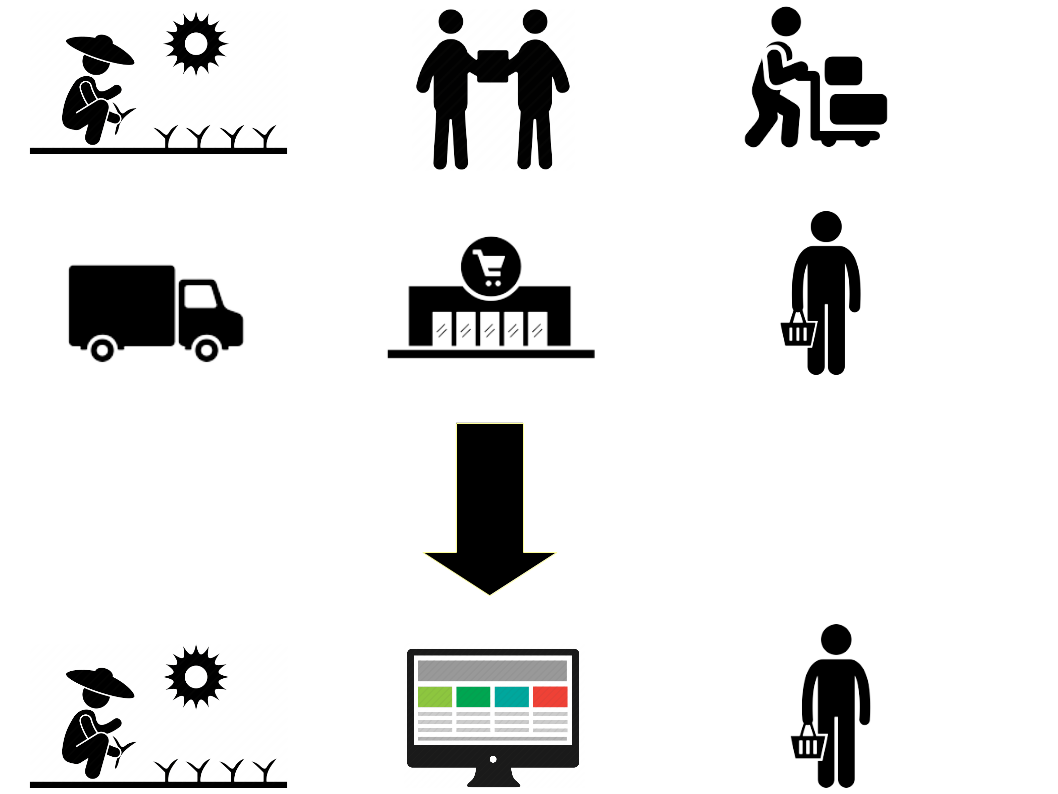
\includegraphics[scale=0.2]{images/chain_production.png}

  \column{\dimexpr\linewidth-40mm-2mm}
    \begin{block}{Consommateurs :}
    Acheter des produits frais et minimiser les étapes de processing.
    \end{block}

    \begin{block}{Producteurs :}
      Maîtriser le prix de vente et les débouchés de leurs productions en se libérant des intermédiaires de distribution.
    \end{block}
\end{columns}
\end{frame}

\begin{frame}{Solution proposée : \texttt{CourtCircuit}}{Problématique et Méthodologie de Résolution}
\begin{block}{Site Web}
Une interface directe entre \textbf{consommateurs} et \textbf{fournisseurs}.
\end{block}

\begin{definition}[Ruche]
Un regroupement de plusieurs \textbf{fournisseurs} d'une région, \textbf{sans guide explicite} préfixé par le site.
\end{definition}

\begin{block}{Vision Décentralisée et Autonome}
\begin{itemize}
  \item l'ensemble des ruches ne répond à \textbf{aucune entité centrale}.
  \item chaque ruche s'occupe de ses propres besoins et de leur gestion sans besoin d'un intermédiaire et d'une hiérarchie à respecter.
\end{itemize}
\end{block}
\end{frame}

\subsection{Méthodes agiles}
\begin{frame}{Méthodologie de résolution : méthodes agiles}{Problématique et Méthodologie de Résolution}
\begin{block}{Méthodes Agiles}
Une approche de développement logiciel de plus en plus prépondérante basée sur une conception/développement itérative, orientée-test et orientée-client.
\end{block}

\begin{block}{Pourquoi ?}
\begin{itemize}
  \item meilleure gestion des ressources
  \item sortie plus fréquente de versions fonctionnelles et testées du produit
  \item interaction plus fréquente avec les clients : adaptation et extensibilité du produit selon leurs besoins
\end{itemize}
\end{block}
\end{frame}
%----------------------------------------------------------------------------------------
%   IMPLEMENTATION
%----------------------------------------------------------------------------------------

\section{Implémentation et résultats}
\subsection{\protect\textit{SPA, Single Page application}}
\begin{frame}{\textit{SPA, Single Page Application}}{Implémentation}
    schema du SPA
\end{frame}

\begin{frame}{\textit{SPA, Single Page Application}}{Implémentation}
    pros et cons du SPA
\end{frame}


\subsection{\protect\textit{Front-end}}
\begin{frame}{\textit{React}}{Front-end}

\end{frame}

\begin{frame}{\textit{Bootstrap et Font-Awesome}}{Front-End}

\end{frame}

\begin{frame}{\textit{Charte Graphique}}{Front-End}

\end{frame}

\subsection{\protect\textit{Back-end}}
\begin{frame}{\textit{Node.js}}{Back-end}

\end{frame}

\begin{frame}{\textit{Express}}{Back-end}

\end{frame}

\begin{frame}{\textit{MariaDB}}{Back-end}

\end{frame}

%----------------------------------------------------------------------------------------
%   CONCLUSION
%----------------------------------------------------------------------------------------
\section{Conclusion}
\subsection{Difficultés survenues}
\begin{frame}{Difficultés survenues}{Conclusion}
    \begin{itemize}
      \item Nouveaux outils nécessitants d'un temps d'apprentissage
      \item Temps dédié à l'implémentation insuffisant
      \item Problème avec le serveur d'hébergement
    \end{itemize}
\end{frame}

\subsection{Perspectives}
\begin{frame}{Perspectives}{Conclusion}

\end{frame}


\subsection{Apports personnels}
\begin{frame}{Apports personnels}{Conclusion}
    \begin{itemize}
      \item Difficulté survenu = Apport personnel
      \item Concepts et technologies utiles appris
      \item Un projet a continuer hors du parcours pédagogique
    \end{itemize}
\end{frame}


\end{document}
